% uitleggen wat, waarom
% veranderingen met mockups
\section{Implementation} \label{implementation}

This section describes the implementation process. The design highlighted the usage of the dashboard through its personas and scenarios, while the low fidelity mockups gave an early glance at its appearance. However, at the heart of this application lies the ability to customize and easily integrate new components. To provide these features, a lot of thought went into choosing the best libraries fit for the job.

First, an overview of the global scope of the application is given, after which we go into more detail. The dashboard consists of two major parts common to web development. The back end is described first. This section covers topics such as the chosen frameworks, the REST API, and data storage. For the front end part, the framework which supports our module-based design and its underlying principles are explained. The contribution of both parts towards a customizable dashboard which allows simple integration, is explained further in their respective sections. It is without question that during the implementation small changes were made to the design. These changes are also documented for both parts. During the entire development process, no effort was put towards privacy safeguards and standard support as they are out of the scope of this thesis.

    % web app, waarom
    % delen van app
    \subsection{Overview}

    The first major choice that was made, was the type of application to develop: a native application or a web application. It was a relative simple choice, but nonetheless an important one. Native applications are developed, in most cases, for one type of operating system. If a developer wants to support both Android and iOS devices, separate applications need to be developed for each of them. Maintaining multiple applications requires a lot more development effort. Java, for example, has the benefit that it is cross-platform thanks to its virtual machine. However, regardless of platform, platform specific changes need to be made to tackle bugs. One of the largest drawbacks of native applications is updating them. This process often requires the reinstallation of the application. As a result, rolling out software updates in hospitals is a difficult task.

    Web applications saw a recent surge in popularity. Web applications today are sometimes very similar in user interface and functionality. An example is Office 365 Web Apps, which shares a lot of functionality from its native counterpart. While these web applications also require updates, these happen on the server side. When the user refreshes the web page, the latest version of the application is automatically loaded. This simplifies the roll-out process significantly. Also, all operating systems that support web browsers, are capable of running this type of applications. As a result, developers only have to develop one version. Mobile devices, therefore, are capable of viewing these applications. However, to fit their small screen, developers need to support a flexible layout.

    With this in mind, the choice to create a web application was evident. Users can view the dashboard regardless of the device they use, without sacrificing functionality. It should be noted that complex image processing applications will not fit easily into the dashboard, due to their computational complexity. Web applications are limited in this regard. Transferring the computational burden to the server side also has the drawback of latency, which the user can experience as slow.

    \begin{figure}[!t]
        \centering
        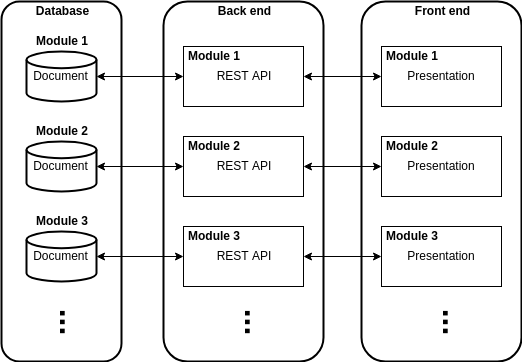
\includegraphics[width=0.9\textwidth]{chapters/4_implementation/structure}
        \caption{The application structure}\label{fig:structure}
    \end{figure}

    A typical web application consists of two parts: the back end and the front end. In software engineering principles, these refer to the separation of the data access layer and the presentation layer of the web application. For example, the back end fetches data requested by the front end. In turn, the front end presents the retrieved data towards the user. Due to the modular design of the dashboard, each module needs to have its own back end (data retrieval and database models) and front end functionality as summarized in figure \ref{fig:structure}.  As seen in the figure, there is no interaction between the modules. Furthermore, the front end has a general presentation in which the modules reside. The next sections describe the back end and front end in detail. Also, before the implementation began, I only had basic knowledge of HTML, CSS, and JavaScript. As a result, the learning curve was personally quite steep.

    % technologie, rest api, nodejs...
    % API reference -> bijlage
    \subsection{Back end}

    The back end consists of a REST API which handles the requests sent by the front end. Each request that the back end supports performs an operation on the database. Examples of such requests are fetching, posting, and deleting data. In this section we describe the REST API, its structure, and the operations it allows. Hereafter, we mention how the database program was chosen, its models and their relations.

        \subsubsection{REST API}

        Node.js was used to create the back end server. This server environment was chosen due its large user base and available libraries. The REST API itself was created with the Express framework and tested with Postman. The documentation of the REST API present in the prototype can be found in appendix \ref{app_rest_api}. We now describe the general structure of the API and the operations it supports.

        \paragraph{General structure} The API structure starts at the user. Each user has a unique identifier which is passed on to the subroutes. To get the information of the user, we send the following request:\\
            \tab\texttt{GET /user/123456}\\
        If there is a user present with the id `123456', the API sends a response containing the user information. Modules that want to use data from a certain user, need to prepend their request with \texttt{/user/id\_value}, as this is the main route. For example, both a heart rate and a blood pressure module want to retrieve their respective values of a certain user whose id is `1a2b3c'. The modules each send the following request:\\
            \tab\texttt{GET /user/1a2b3c/heart}\\
            \tab\texttt{GET /user/1a2b3c/bp}\\
        Each module is responsible for its own subroutes and operations it supports. As an example, the threshold values can be retrieved differently for each module, depending on the developer's choice:\\
            \tab\texttt{GET /user/1a2b3c/heart/thresholds}\\
            \tab\texttt{GET /user/1a2b3c/bp/misc\_values/thresholds}\\
        The subroutes are simple to integrate thanks to the Express framework. All the requests a subroute handles are stored in its own file. The main route imports this file so it can forward the subroute towards that module. Suppose we have a \texttt{route/heart.js} file that we want to integrate in the main route \texttt{user.js}. This is done as follows:\\
            \tabsmall\texttt{const heartRoutes = require('.routes/heart'); //import routes}\\
            \tabsmall\texttt{router.use('/:userId/heart', heartRoutes); //forward routes}\\
        Only two lines are needed to import all the necessary requests from a module. The main route, and all subroutes of all modules present in the prototype are documented in appendix \ref{app_rest_api}.

        \paragraph{Operations}
        The modules can create new, retrieve, delete, and update data entries. Respectively, these are the following request types: POST, GET, DELETE, and PATCH. In the prototype however, data deletion is not possible because it concerns valuable medical data. For threshold values, deletion is also not possible as every patient is required to have these. Creation of the thresholds for a patient is only possible there is currently no entry present for that patient. Again, appendix \ref{app_rest_api} documents all implemented operations for all modules present in the prototype.

        \subsubsection{Database}

        MongoDB was chosen as the database program, which uses JSON-like documents to store data. Groups of these documents are stored in collections. A feature of MongoDB is that the documents inside a collection do not need the same data fields. Suppose we update our patient information page to also show their phone number. In SQL, tables would need to be redefined and the existing rows updated to have a default value for this attribute. In MongoDB this is not necessary as  patients with this new attribute can be added without a problem to the existing collection. These flexible documents facilitate integration as no schema rules need to be defined. This allows developers to create their own document schemas and pair them to existing users by solely referring to their id.

        \begin{figure}[!t]
            \centering
            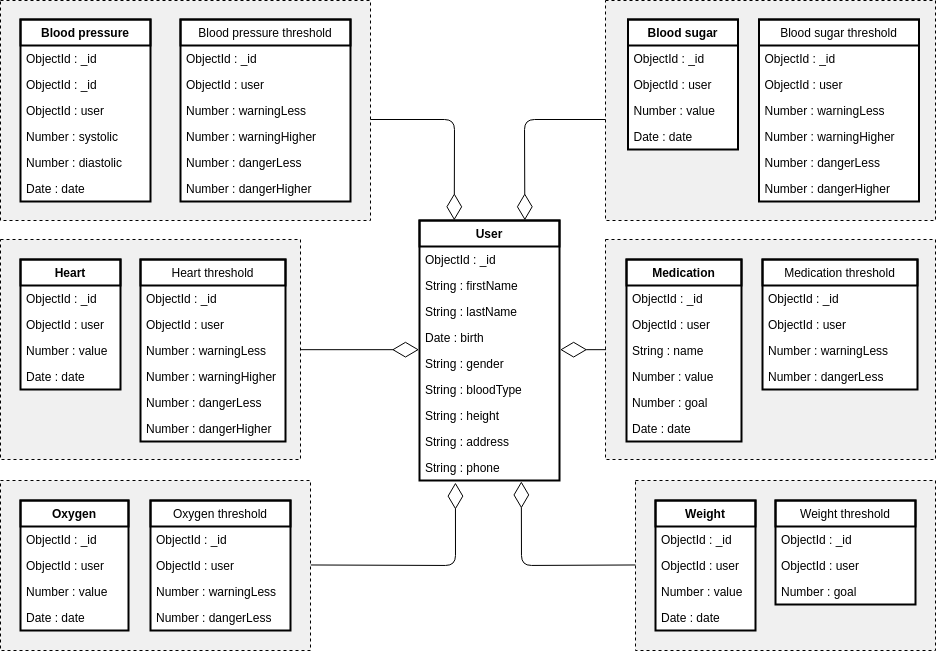
\includegraphics[width=1.0\textwidth]{chapters/4_implementation/db}
            \caption{The database structure}\label{fig:db}
        \end{figure}

        The prototype runs a local MongoDB database server where all dashboard data is stored. Each module is responsible for its own documents. As such, every module has a value collection, which contains all values of all users, and a threshold collection, where one threshold entry exists for each user in the dashboard system. No module accesses data from another module. The database is managed via the Mongoose modeling library for Node.js. By defining models, Mongoose helps us by managing relationships between data. Also, it translates source code objects to their representation in the database.

        

        The models present in this prototype are straightforward, as shown in figure \ref{fig:db}. It is possible that one blood pressure entry can have an additional field, such as whether it was seen or not by the clinician. However, the current implementation of each module, ignores extra data fields. If in the future data fields are added, the front end part of the module must adapted in order to present these to the clinician.

    % technologie
    % screens -> rest bijlage
    % veranderingen met mockups
    \subsection{Front end}

    Ultimately, the front end is what the user sees. From the onset of the implementation process, the search for a library which supports a modular approach began. It was clear that Web Components would be used to create the individual modules, which will be explained in the next section. There are several libraries that support the creation of Web Components. Google's Polymer library was eventually chosen, due to its extensive documentation. The following sections describe the Web Component principles and the structure of the front end. For the latter, the customization aspect and the library used to achieve this are explained.

        \subsubsection{Web Components}
        
        \begin{figure}[!t]
            \centering
            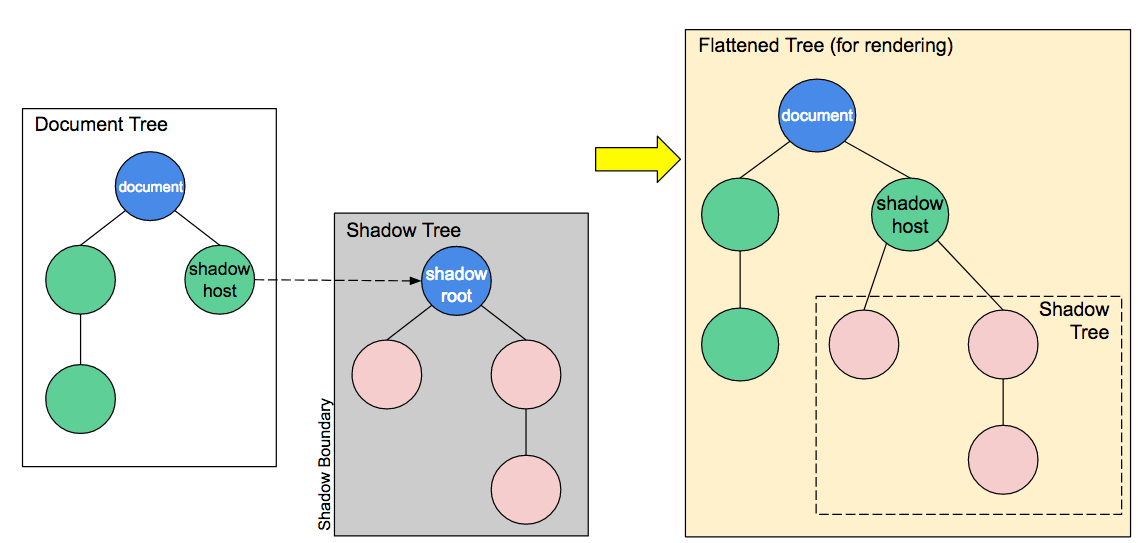
\includegraphics[width=1.0\textwidth]{chapters/4_implementation/shadow-dom}
            \caption{The shadow DOM (src: \url{https://developer.mozilla.org/en-US/docs/Web/Web_Components/Using_shadow_DOM})}\label{fig:shadow_dom}
        \end{figure}

        HTML provides us with standard elements such as \texttt{h1} and \texttt{img}. Web Components allows the developer to create custom elements which can be used in the same manner as the ones HTML provides. Suppose a calendar Web Component was created, a developer could add the element to any web page as follows: \texttt{<calendar></calendar>}. The actual definition of the calendar module resides in another file which is imported on the page where it will be used. This approach supports reusability, and above all, easy integration which is a primary goal of our dashboard application. At the heart of Web Components is the shadow DOM.

        \paragraph{Shadow DOM} We assume the reader is familiar with the DOM concept. The shadow DOM can be seen as a scoped subtree inside a custom element. The root of this subtree is called the shadow root. The structure, styling, and behavior of the children within the shadow DOM do not affect any elements outside of it. Therefore, the appearance and functionality of the custom element is encapsulated and hidden at the document level. Only events fired by elements in the shadow DOM can be pickup outside the shadow DOM boundary. Figure \ref{fig:shadow_dom} visualizes this concept. This idea of encapsulation is important for our approach toward the dashboard, as each module is responsible for its own appearance and functionality. Developers of custom modules should not need to worry about what happens outside of the shadow DOM.

        \subsubsection{Structure}

        \begin{figure}[!t]
            \centering
            \frame{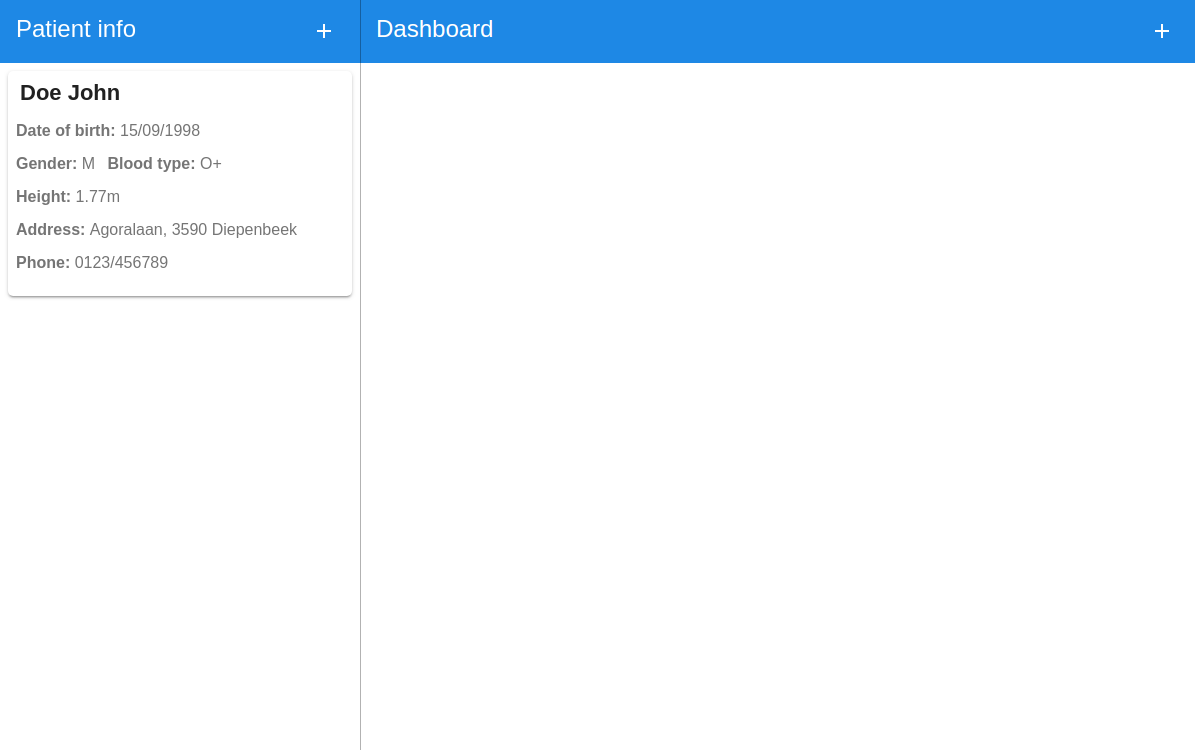
\includegraphics[width=1.0\textwidth]{screenshots/db_empty}}
            \caption{The empty dashboard}\label{fig:screen_db_empty}
        \end{figure}

        The dashboard features two panels. On the left, only small modules can be pinned, while both the small and large modules can be placed on the right panel. The left panel is thin and can be hidden in case of small screen estate. Should too many modules be present on the right pane, scrolling is possible. The left pane will stay in place to still show the information of the small modules that reside there. Figure \ref{fig:screen_db_empty} shows the empty dashboard.

        The right panel allows the ordering of the modules via drag-and-dropping them into place. Several libraries were tried out to achieve this functionality, but many of them did not support dragging elements within a shadow DOM. As a result, the front end was rebuilt several times. Eventually, Packery.js was used. This library allows free placement of the modules and tries to arrange them to maximize space efficiency. In case of resizing, the modules are rearranged automatically. Modules are added through a dialog which can be accessed by pressing the plus-sign button in the top-right corner. The same applies for the smaller panel on the left side. However, the modules in this panel can only be realigned vertically.

    \subsection{Result}

    